\documentclass[main.tex]{subfiles} % Subfile-Class

%==============================================================================%
%                                   Subfile                                    %
%==============================================================================%

\begin{document}

% Template

\section{Linienfolger - Reglerauslegung und Parametrierung}~\label{apdx:LineFollowerRegler}

\subsection*{Liniensensor Funktionsweise}~\label{apdx:Liniensensor_auswertung}

Der Liniensensor wurde, wie bereits in PREN1 ausführlich dokumentiert, mit acht
Helligkeitssensoren realisiert. Die Idee ist, dass diese Sensoren, die im
sichtbaren Lichtspektrum empfindlich sind, die Floureszens des Klebebandes
auswerten. Da das Klebeband mit UV-Licht bestrahlt wird, fluoresziert es stark
und bildet damit einen deutlichen Kontrast zur Bodenfuge beziehungsweise zu den
Fliesen des Wettkampfbodens.

% TODO: Abbildung

Der Vorwiderstand der Messzellen ist so dimensioniert, dass der
lichtempfindliche Transistor in Sättigung geht, sobald sich eine Linie
unterhalb des Sensors befindet. Dadurch wird der starke Kontrast auch in der
Spannung über der Messzelle deutlich sichtbar.

\subsection*{Sensor Auswertung}

\paragraph{Auslesen und normieren der Werte}

Der Sensor wird analog über einen A/D-Wandler ausgelesen. Die acht Messwerte
werden in einem Array gespeichert.

Anschliessend werden alle Messwerte auf einen Bereich zwischen $0 \dots 1000$
normiert. Dazu sind Kalibrationswerte für die Maximal- und Minimalspannungen
($Calib_{\max}$ und $Calib_{\min}$) erforderlich, welche für jede Zelle
individuell durch Messungen auf dem Wettkampfboden ermittelt sind.

Die Firmware des MotionControllers implementiert ausserdem eine
Kalibrierungsroutine, bei welcher passende Werte möglichst aktuell ermittelt
werden können. Dazu wird jede Sensorzelle auf den verschiedenen Untergründen
Fliese und Klebeband automatisch 50 mal hintereinander ausgelesen und im
Anschluss der entsprechende Median als Kalibrierungswert gespeichert.

\[
    Val_{norm} = (Val_{raw} - Calib_{\min}) \cdot \frac{1000}{Calib_{\max} - Calib_{\min}}
\]

\paragraph{Gewichtetes Summieren der Werte}
Ziel ist es, die Linienposition in Form einer einzelnen Zahl auszugeben. Dazu
werden die normierten Sensorwerte herangezogen, und gewichtet zusammengezählt.

\[
    LinePos = \frac{0 \cdot Val_{norm}[0] + 1 \cdot Val_{norm}[1] + \cdots + 7 \cdot Val_{norm}[7]}{\sum_{k=0}^{7}(Val_{norm}[i])}
\]

Ergibt die Berechnung $0$ oder $7000$, so befindet sich die Linie am äusseren
Anschlag. Befindet sich die Linie in der Mitte, ergibt die Berechnung $3500$,
was auch der Sollwert des Linienfolgers ist.

\subsection*{Sensorrauschen}~\label{apdx:Liniensensor_rauschen}

Die Messwerte des Liniensensors zeigen ein deutliches Rauschen. Deutlich ist
dieses im nachfolgenden Abschnitt in Abbildung~\ref{fig:Sprungantwort}
sichtbar. Um dieses näher zu untersuchen, wurde von den vorhandenen Daten
(siehe Abbildung \ref{fig:FFT_START}) eine FFT (Fast-Fourier-Transformation)
erstellt. Dabei ergab sich – abgesehen von der Prozessfrequenz, die durch die
Sprungantwort bedingt ist – keine aussergewöhnliche Störfrequenz.

\begin{figure}[H]
    \centering
    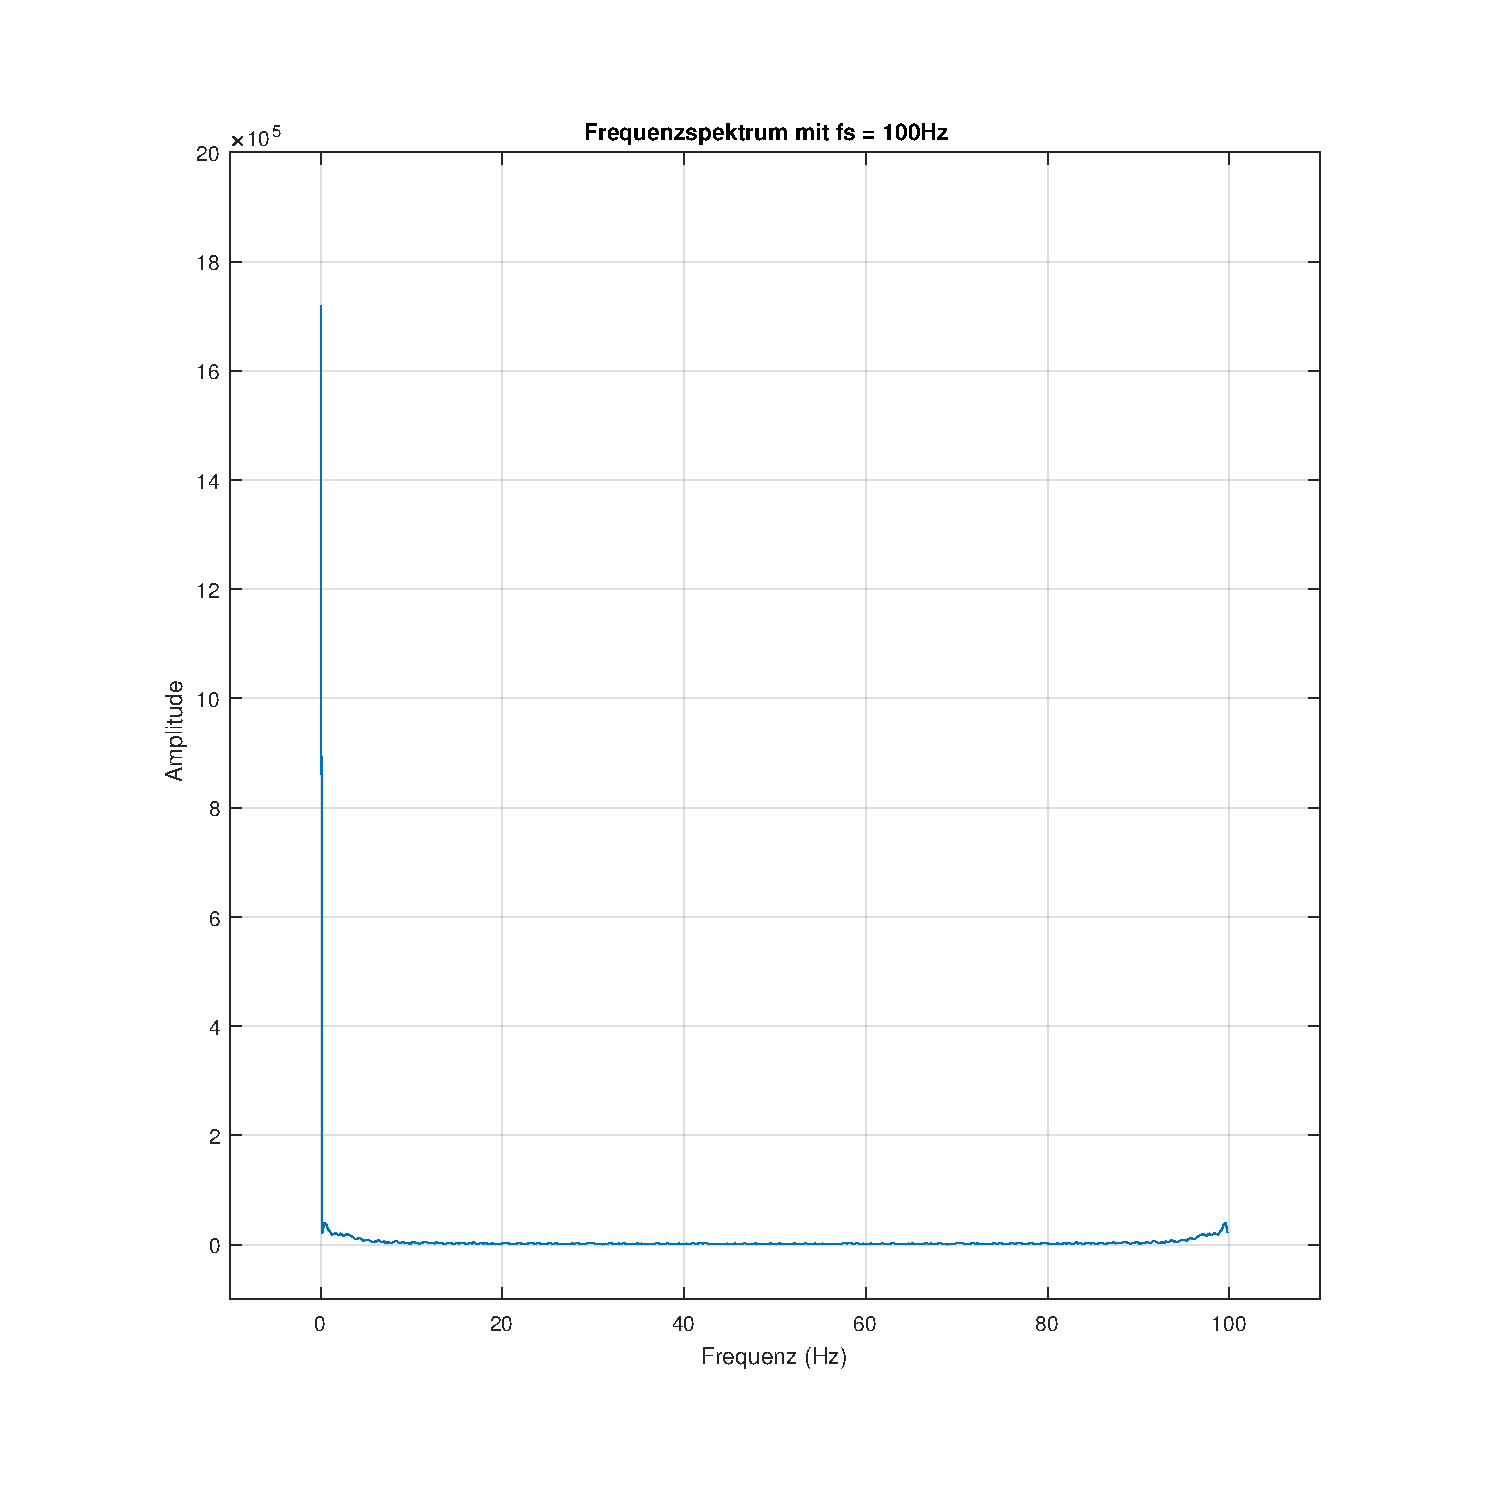
\includegraphics[width=0.5\linewidth]{fig_Parametrierung_Linienfolgeregler/FFT_START.pdf}
    \caption{FFT einer Linienpositions-Messreihe mit Sprungantwort}~\label{fig:FFT_START}
\end{figure}

Eine Messung der ausgegebenen Linienposition im Stillstand des Fahrzeugs
bestätigt, dass der Sensor an sich mit einer Standartabweichung von gerade
einmal $\sigma = 0.6981$ in anbetracht seiner Auflösung sehr genau ist. Bei den
insgesamt $9000$ Messungen ereigneten sich auch keine Ausreisser.

Damit liegt die Erklärung des Messrauschens auf der Linienposition beim
Fahrzeug selbst, welches durch das starre Fahrwerk und die Kugel, welche am
vorderen Ende des Fahrzeugs über den Boden geschliffen wird, einfach stark
vibriert und damit die Messwerte des Liniensensors verunreinigt.

Mit dem Rauschen kann umgegangen werden, es muss allerdings bei der auslegung
des Reglers berücksichtigt werden. Ein allenfalls geplanter D-Anteil darf nicht
zu gross gewählt werden, da sich das Rauschen sonst im Systemverhalten zeigen
wird.

\subsection*{Sensor-Grenzwerte für die Liniendetektion}\label{apdx:Liniensensor_Liniendetektion}

Über den Liniensensor ist das System in der Lage, zwischen Fliese, Fuge und Klebeband
zu unterscheiden. Über die Funktion und das Rauschverhalten wurde bereits viel
berichtet. Dieser Abschnitt beschäftigt sich mit der Frage, wie diese Unterschiede genau
festgestellt werden können und wo diese Grenzwerte liegen.

Dazu wurde eine Messreihe auf verschiedenen Untergründen aufgezeichnet. Nachdem
der Liniensensor zuvor mit dem Klebeband-Untergrund und der Fliese sorgfältig
kalibriert wurde, ergeben sich die drei Häufigkeitsverteilungen, die in
Abbildung~\ref{fig:Histogramme_LineSensor} dargestellt sind.

\begin{figure}[H]
    \centering
    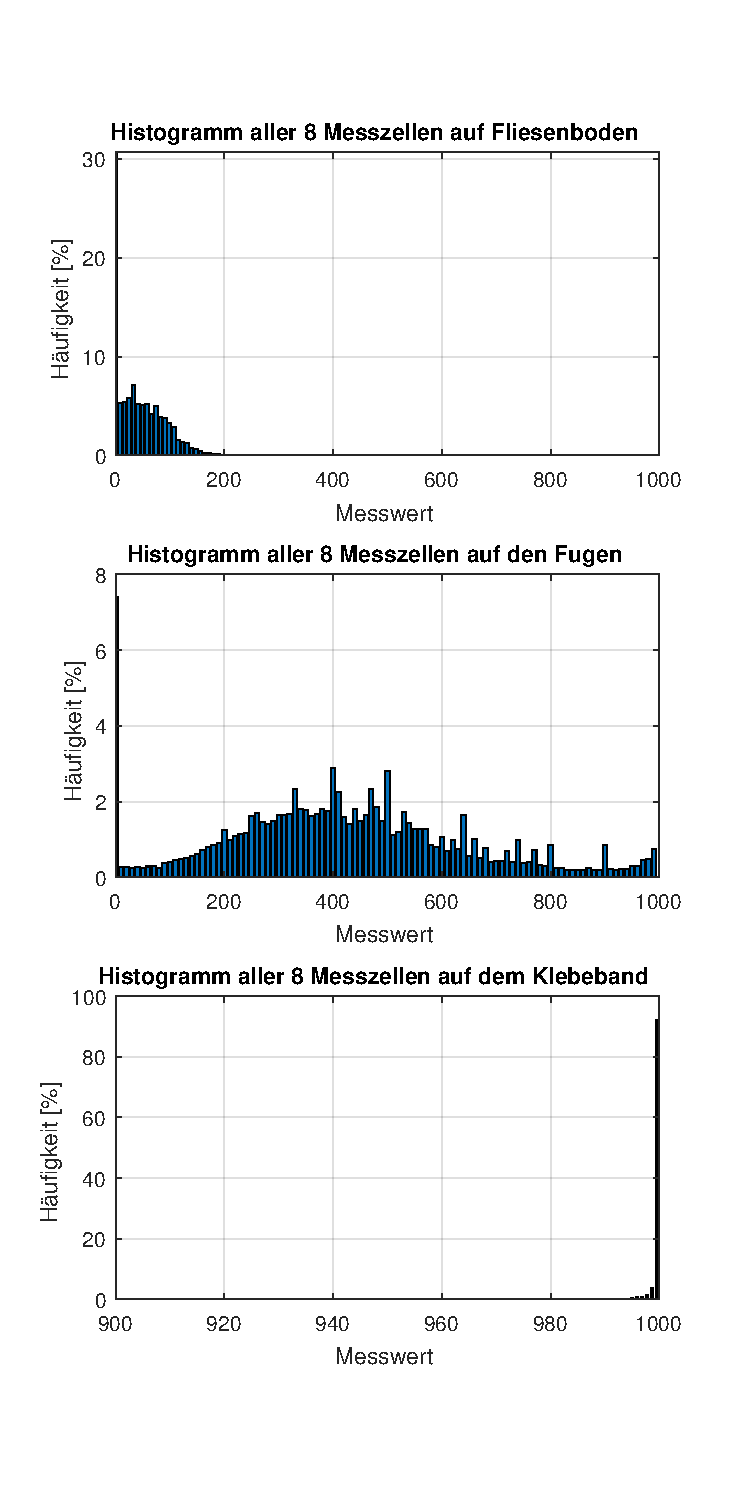
\includegraphics[width=0.5\linewidth]{fig_Parametrierung_Linienfolgeregler/Histogramme_Liniensensor.pdf}
    \caption{Häufigkeitsverteilungen des Liniensensors bei verschiedenen Untergründen}\label{fig:Histogramme_LineSensor}
\end{figure}

Es ist erkennbar, dass sich Klebeband und Fliese sehr deutlich voneinander
unterscheiden lassen. Bei der Detektion der Fuge ist der Unterschied leider
nicht so ausgeprägt wie erhofft. Nichtsdestotrotz sammeln sich die
gaussverteilten Messwerte rund um einen Mittelwert von ca. 420.

Da das Klebeband praktisch ausschliesslich sicher ab einem Wert von 900 als
solches erkannt werden kann, wird der Grenzwert für die Liniendetektion
ebenfalls auf diesen hohen Wert festgelegt. Die Gaussverteilung der Messwerte
erlaubt es, die Wahrscheinlichkeit zu berechnen, mit der eine Fugenmessung
fälschlicherweise als Linie erkannt wird. Diese wird durch das Integral der
Glockenkurve ab eben diesem Punkt ermittelt:

\[
    P(X > n) = 1 - \frac{1}{2} \Bigg( 1 + \operatorname{erf}\!\Bigg( \frac{n - \mu}{\sigma \sqrt{2}} \Bigg) \Bigg)
\]

Die Standardabweichung der Messwerte beträgt \(\sigma = 232.6287\) und der
Mittelwert der Messungen \(\mu = 418.363\). Damit beläuft sich die
Wahrscheinlichkeit, dass eine Fuge fälschlicherweise als Linie erkannt wird,
auf \(1.9207\%\). Dies erscheint zunächst hoch. Allerdings bezieht sich diese
Wahrscheinlichkeit auf einzelne Messungen. Linien sollen jedoch vor allem als
solche erkannt werden, um Knotenpunkte zu identifizieren oder um an einem
Knotenpunkt zu prüfen, ob es sich bei einem Linienabgang tatsächlich um eine
solche handelt. Werden in diesen Szenarien statt einer Messung gleich 5
Messungen durchgeführt, reduziert sich die Wahrscheinlichkeit für eine falsch
detektierte Linie bzw. einen falsch detektierten Knotenpunkt auf \(P^5 =
0.000026\%\) --- was wiederum ein akzeptables Risiko darstellt.

Die gleiche Überlegung lässt sich auch auf das Szenario übertragen, in dem das
Fahrzeug über eine Fuge fährt, die in unmittelbarer Nähe der Linie verläuft.
Fährt das Fahrzeug mit 0,5\,m/s, so überquert es die Fugenbreite von 50\,mm in
5 Messzyklen. Die Wahrscheinlichkeit, dass die Fuge nach diesen 5 Messzyklen
noch immer als Linie interpretiert wird, ist derart gering, dass dieses
Restrisiko in Kauf genommen wird.

Die Problematik, dass eine Fuge fälschlicherweise als Linie erkannt wird, zeigt
sich nur in Situationen in denen über eine Quer verlaufende Fuge gefahren wird
und damit ein Knotenpunkt erkannt werden könnte. Verläuft eine Fuge nahe und
paralell zu einer Linie, bezweckt das gewichtete Aufsummieren, dass die
Linienposition sich sehr stark nach der \textit{hellsten} Sensorzelle richtet.
Das ist, auch wenn eine Fuge paralell verläuft, immer das Klebeband.

% ---------- REGLER -------------------

\subsection*{Regler Aufbau}

\begin{figure}[H]
    \centering
    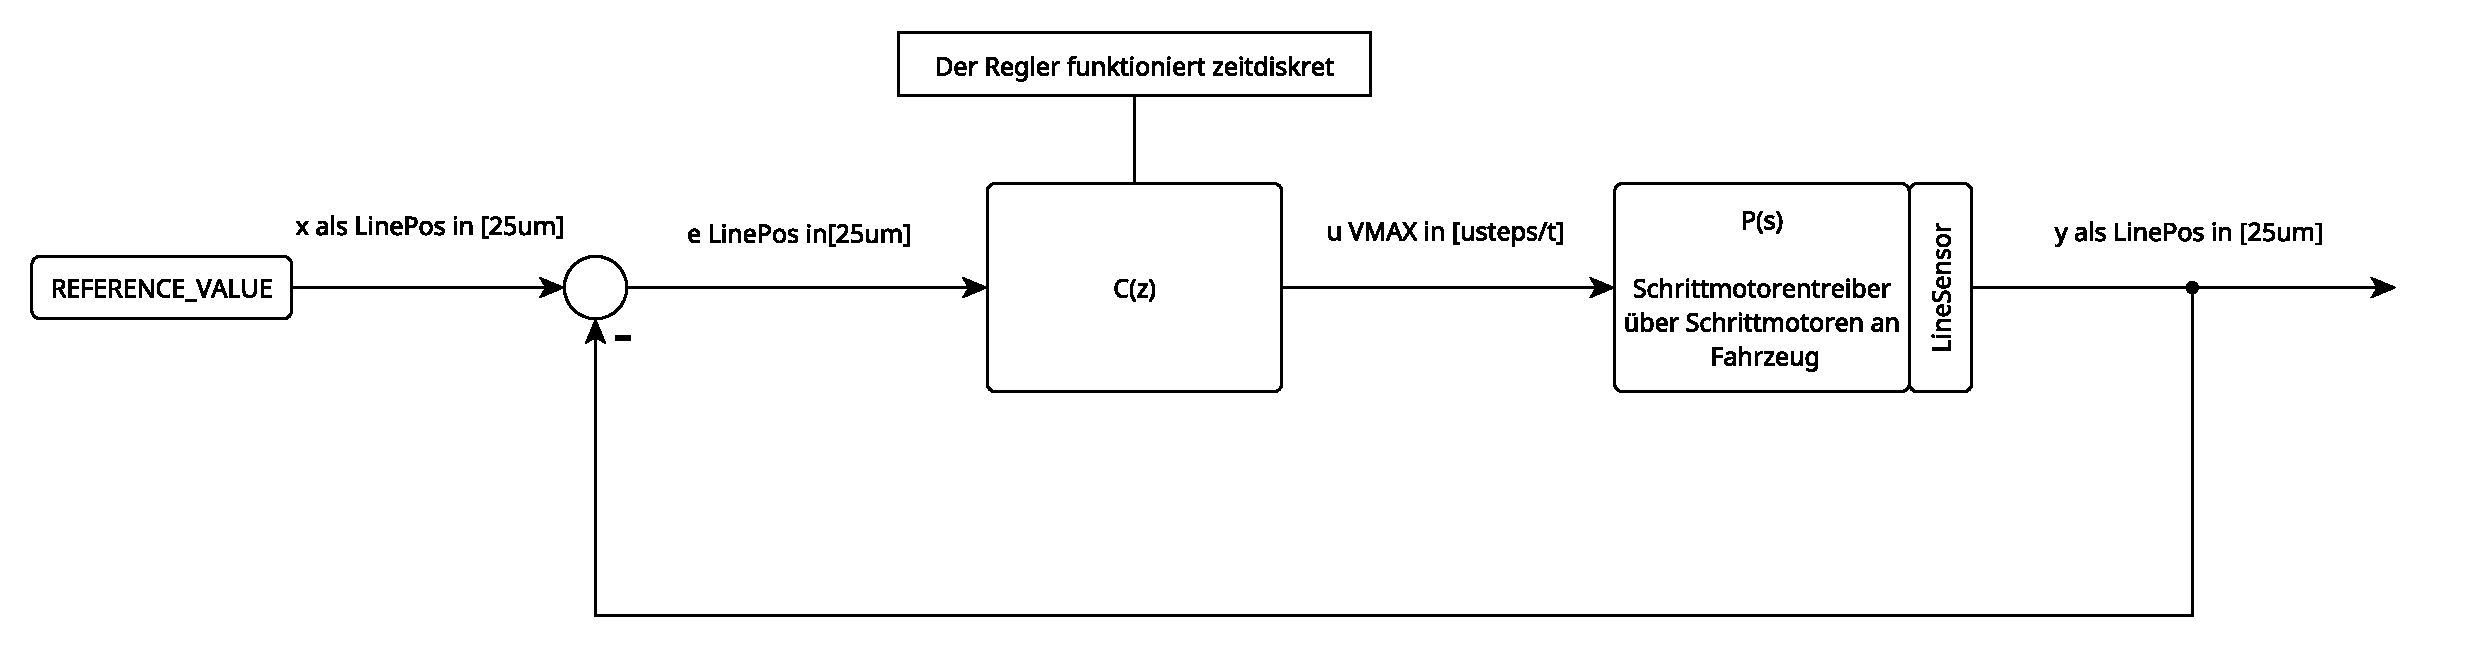
\includegraphics[width=1.0\linewidth]{fig_Parametrierung_Linienfolgeregler/RegelProzess_Linienfolger.pdf}
    \caption{Reglerprozess des Linienfolgers}~\label{fig:Linienfolger_RegelProzess}
\end{figure}

Die Abbildung~\ref{fig:Linienfolger_RegelProzess} zeigt schematisch, wie der
Regelprozess funktioniert. Eingangsgrösse ist die Bezugsgrösse $x$, die im
vorhergehenden Abschnitt auf die konstante Linien-Mittenposition $3500$
festgelegt ist. Diese Grösse gibt die auf den Messzellenabstand aufgelöste
Linienposition auf einer Skala von $0 \dots 7000$ an und hat die Einheit $25\mu
    m$.

Der zeitdiskrete Regler $C(z)$ implementiert einen zeitdiskreten PD-Regler,
dessen Parametrierung im folgenden Abschnitt \textit{Reglerparametrierung}
näher erläutert wird. Die Ausgangsgrösse $u$ des Reglers entspricht der
Motordrehzahl in $\frac{\mu \text{steps}}{t}$, die im Prozess $P(s)$ durch die
Motortreiber in eine Fahrbewegung umgesetzt wird.

Der Prozess $P(s)$ beschreibt das gesamte Verhalten des Fahrzeugs. Dies umfasst
den Regelkreis von der Ausgabe der Fahrsignale an die Motortreiber über das
gesamte Fahrverhalten bis hin zur erneuten Auswertung der Streckenlage über den
Liniensensor. Dementsprechend ist die Ausgangsgrösse dieses Prozesses $y$
wieder die Linienposition, die am Eingang des Reglers mit der Referenzgrösse
verglichen wird, um den Regelfehler $e$ zu bestimmen.

\subsection*{Regler Parametrierung}~\label{apdx:Regler_Parametrierung}

\subsubsection*{Aufzeichnung der Sprungantwort und Prozessmodellierung}

Um das Fahrverhalten zu analysieren, ist ein einfacher P-Regler implementiert.

\[
    C(z) = k_p \cdot e(z)
\]

Der Parameter $k_p = 5$ wurde so gewählt, dass das Fahrzeug Fahrfehler über
eine längere Strecke einigermassen kompensieren kann. Um eine Sprungantwort
aufzuzeichnen, wird dem Fahrzeug ein Sprung in Form eines Klebebandes
vorgesetzt und der Ausgang des Liniensensors via USB-CDC Schnittstelle
ausgegeben.

\begin{figure}[H]
    \centering
    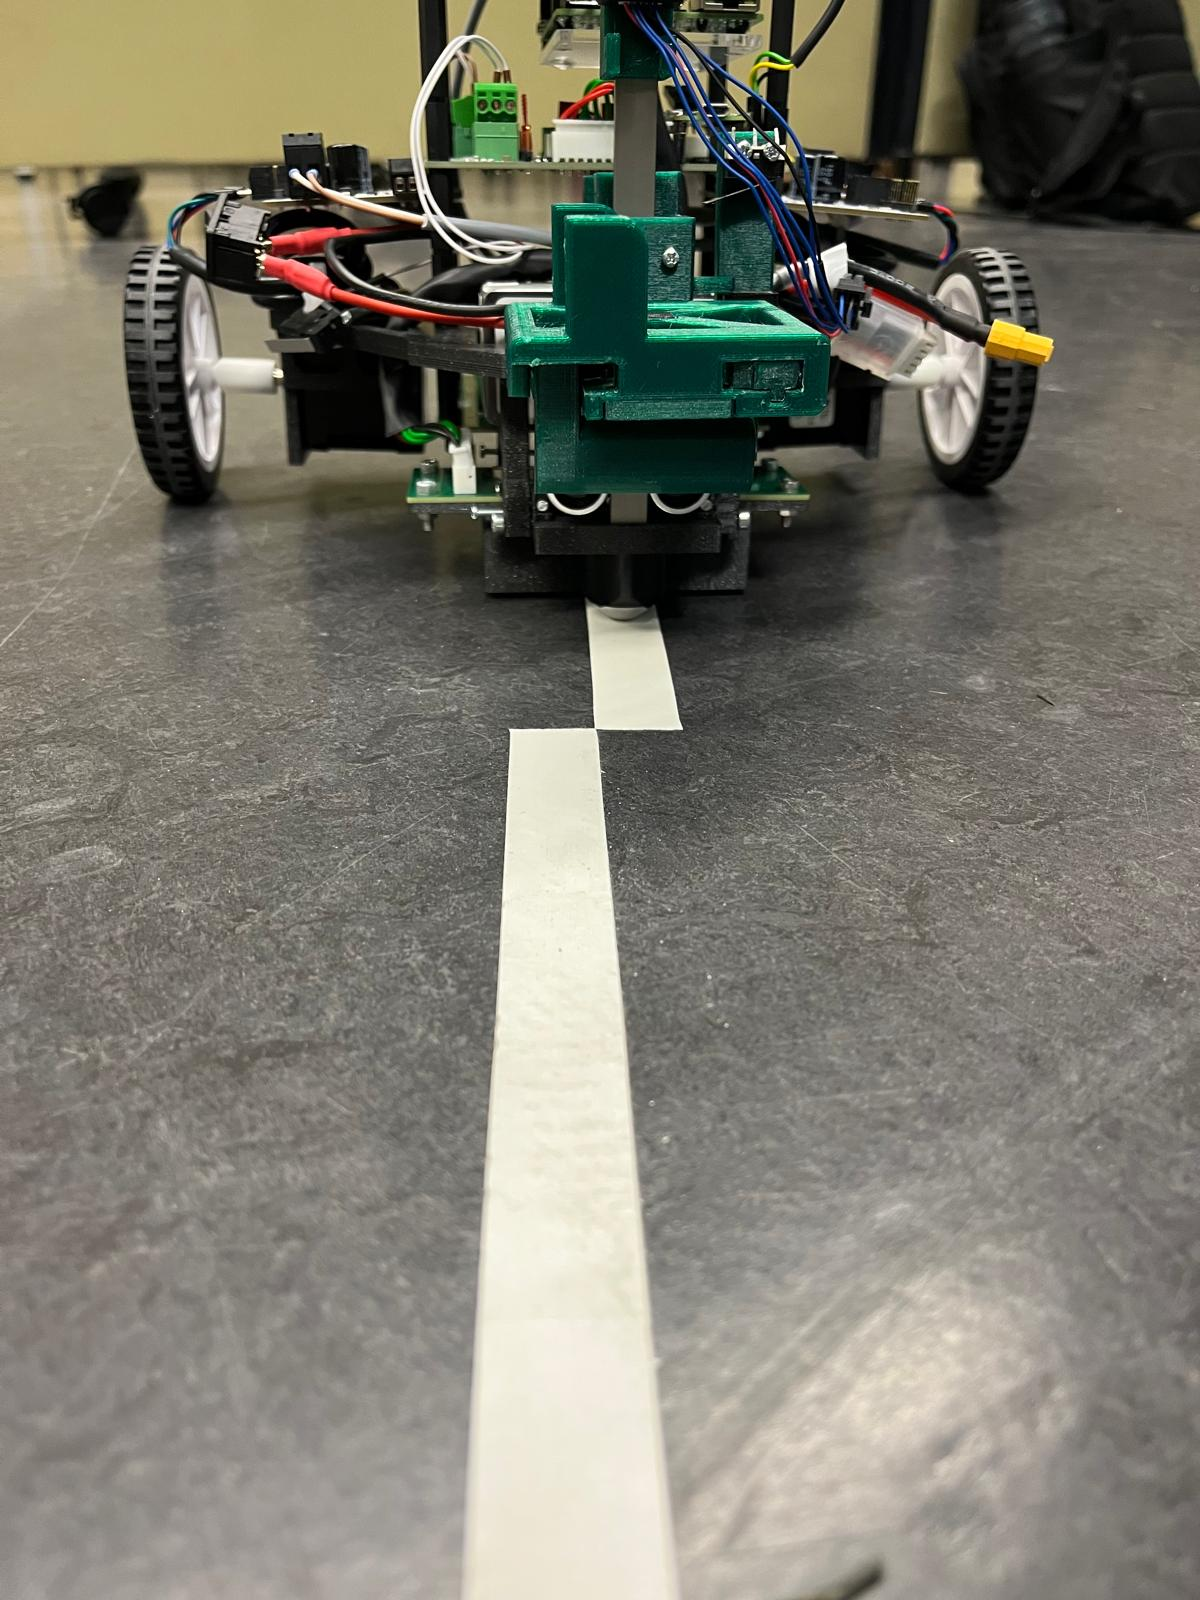
\includegraphics[width=1\linewidth]{fig_Parametrierung_Linienfolgeregler/Versuchsaufbau_Sprungantwort.jpeg}
    \caption{Versuchsaufbau zum Aufzeichnen der Sprungantwort}~\label{fig:Linienfolger_Versuchsaufbau_Sprungantwort}
\end{figure}

Abbildung~\ref{fig:Linienfolger_Versuchsaufbau_Sprungantwort} zeigt den
entsprechenden Versuchsaufbau. Mit Hilfe von Matlab kann nun das
Fahrzeugverhalten grafisch dargestellt werden.

Die gemessene Grösse des Liniensensors entspricht jedoch nicht direkt der
Sprungantwort selbst, sondern vielmehr der aktuellen Abweichung von dieser. Aus
dem Wert des Liniensensors kann somit der aktuelle Regelfehler $e[k]$ abgelesen
werden.

Wird dieser Fehler mit einem Referenzsignal verglichen, das einen Sprung von
der Mittelposition auf etwa $50mm$ beschreibt, lässt sich die tatsächliche
Sprungantwort ableiten.

\begin{figure}[H]
    \centering
    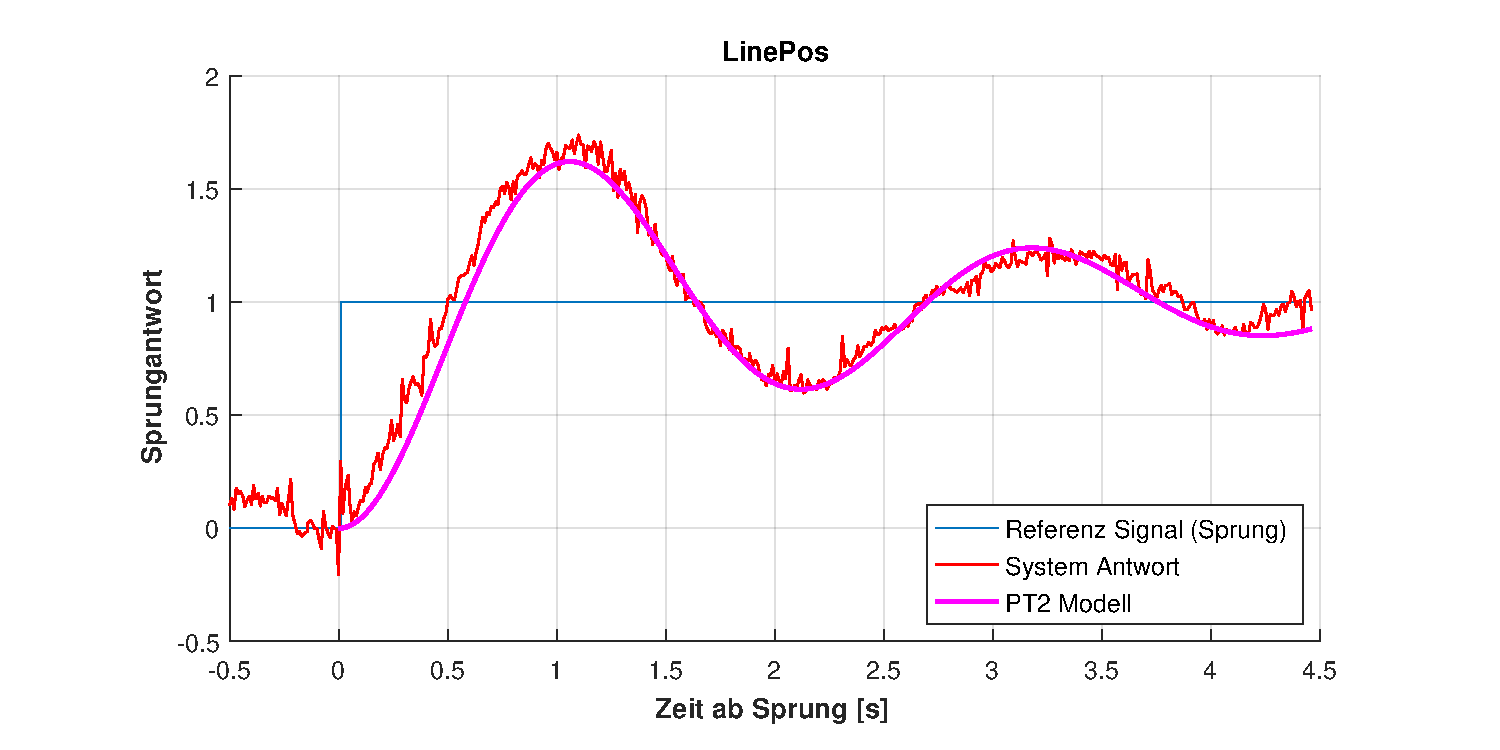
\includegraphics[width=1\linewidth]{fig_Parametrierung_Linienfolgeregler/Sprungantwort_System.pdf}
    \caption{Sprungantwort und PT2 Modell}~\label{fig:Sprungantwort}
\end{figure}

Abbildung~\ref{fig:Sprungantwort} zeigt das Ergebnis dieses Experiments. Die
rote Linie stellt die aufgezeichnete Sprungantwort dar, die magentafarbene
Linie das zugehörige PT2-Modell.

Die Sprungantwort zeigt, dass das System sehr direkt reagiert und praktisch
keine erkennbare Totzeit aufweist. Um die Modellierung zu vereinfachen, wird
davon ausgegagen, dass sich das System tatsächlich wie ein PT2-System ohne
Totzeit verhält.

Das gezeigte Modell besitzt die folgenden Parameter:

\begin{itemize}
    \item $kp = 1$
    \item $\omega = 3.0 rad$
    \item $\zeta = 0.15$
\end{itemize}

Daher, dass der eingesetzte Regler $C(z)$ mit seinem Verstärkungsfaktor $kp =
    5$ bekannt ist, lässt sich aus dieser Closed-Loop Systemantwort der Prozess
$P(s)$ algebraisch ermitteln.

\[
    P(s) \approx \frac{G_{PT2}}{1 - G_{PT2}}
\]

Mit $G_{PT2}$, der Closed-Loop Systemantwort, dargestellt durch das PT2-Modell.
Die Übertragungsfunktion des Prozesses $P(s)$ ergibt sich somit zu
\[
    P(s) \approx \frac{1.8}{s \cdot (s + 0.9)}
\]

\subsubsection*{Auswertung des Prozesses und Anforderung an den Regler}

An der Übertragungsfunktion des Prozesses P sieht man bereits, dass sich das
der Prozess ein integrierendes Verhalten zeigt. Dies ist bereits ein erstes
Indiz dafür, dass von einem zusätzlichen Integralanteil im Regler abgesehen
werden kann.

\begin{figure}[H]
    \centering
    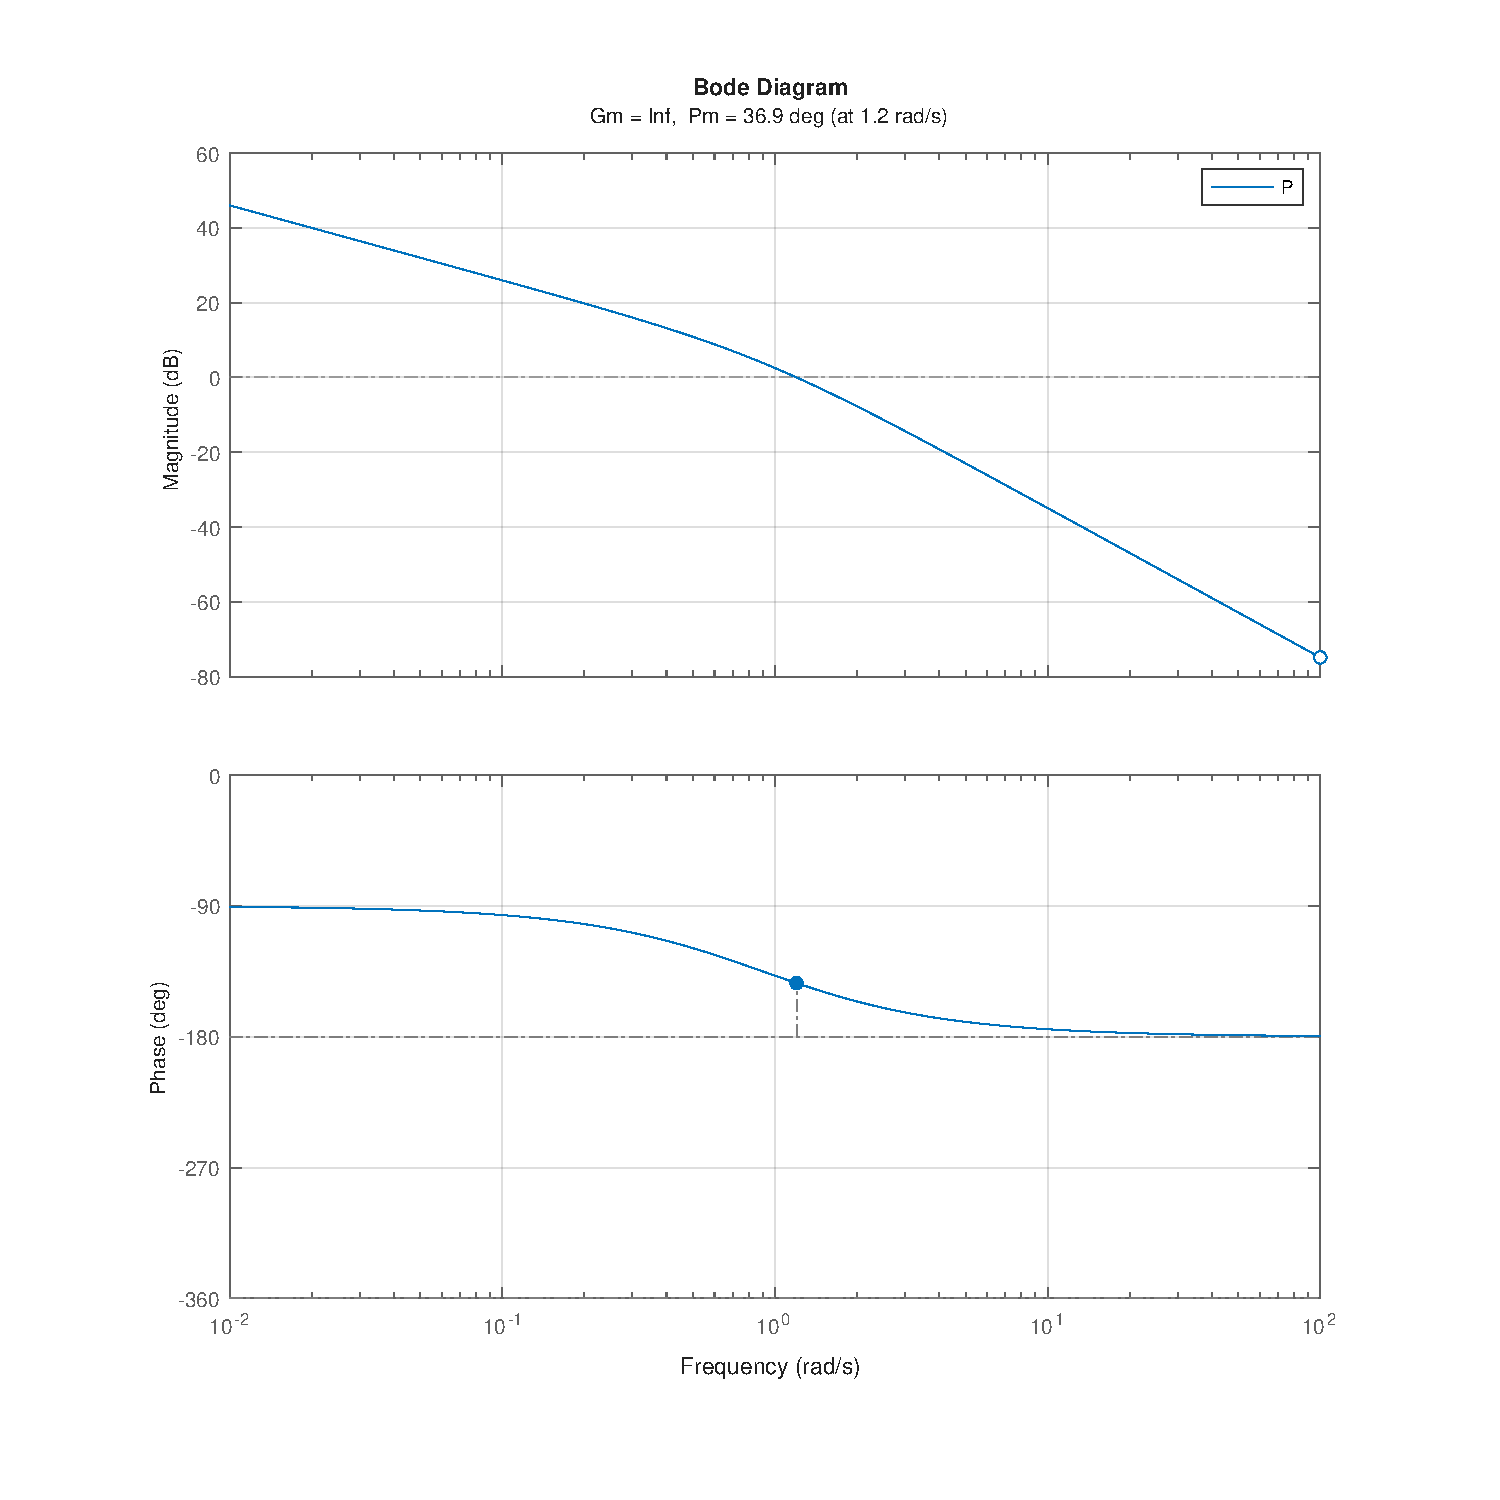
\includegraphics[width=1\linewidth]{fig_Parametrierung_Linienfolgeregler/Bode_Plot_Prozess.pdf}
    \caption{Bodeplot mit eingezeichnter Phasen- und Amplitudenreserve}~\label{fig:MarginPlot_raw}
\end{figure}

\begin{figure}[H]
    \centering
    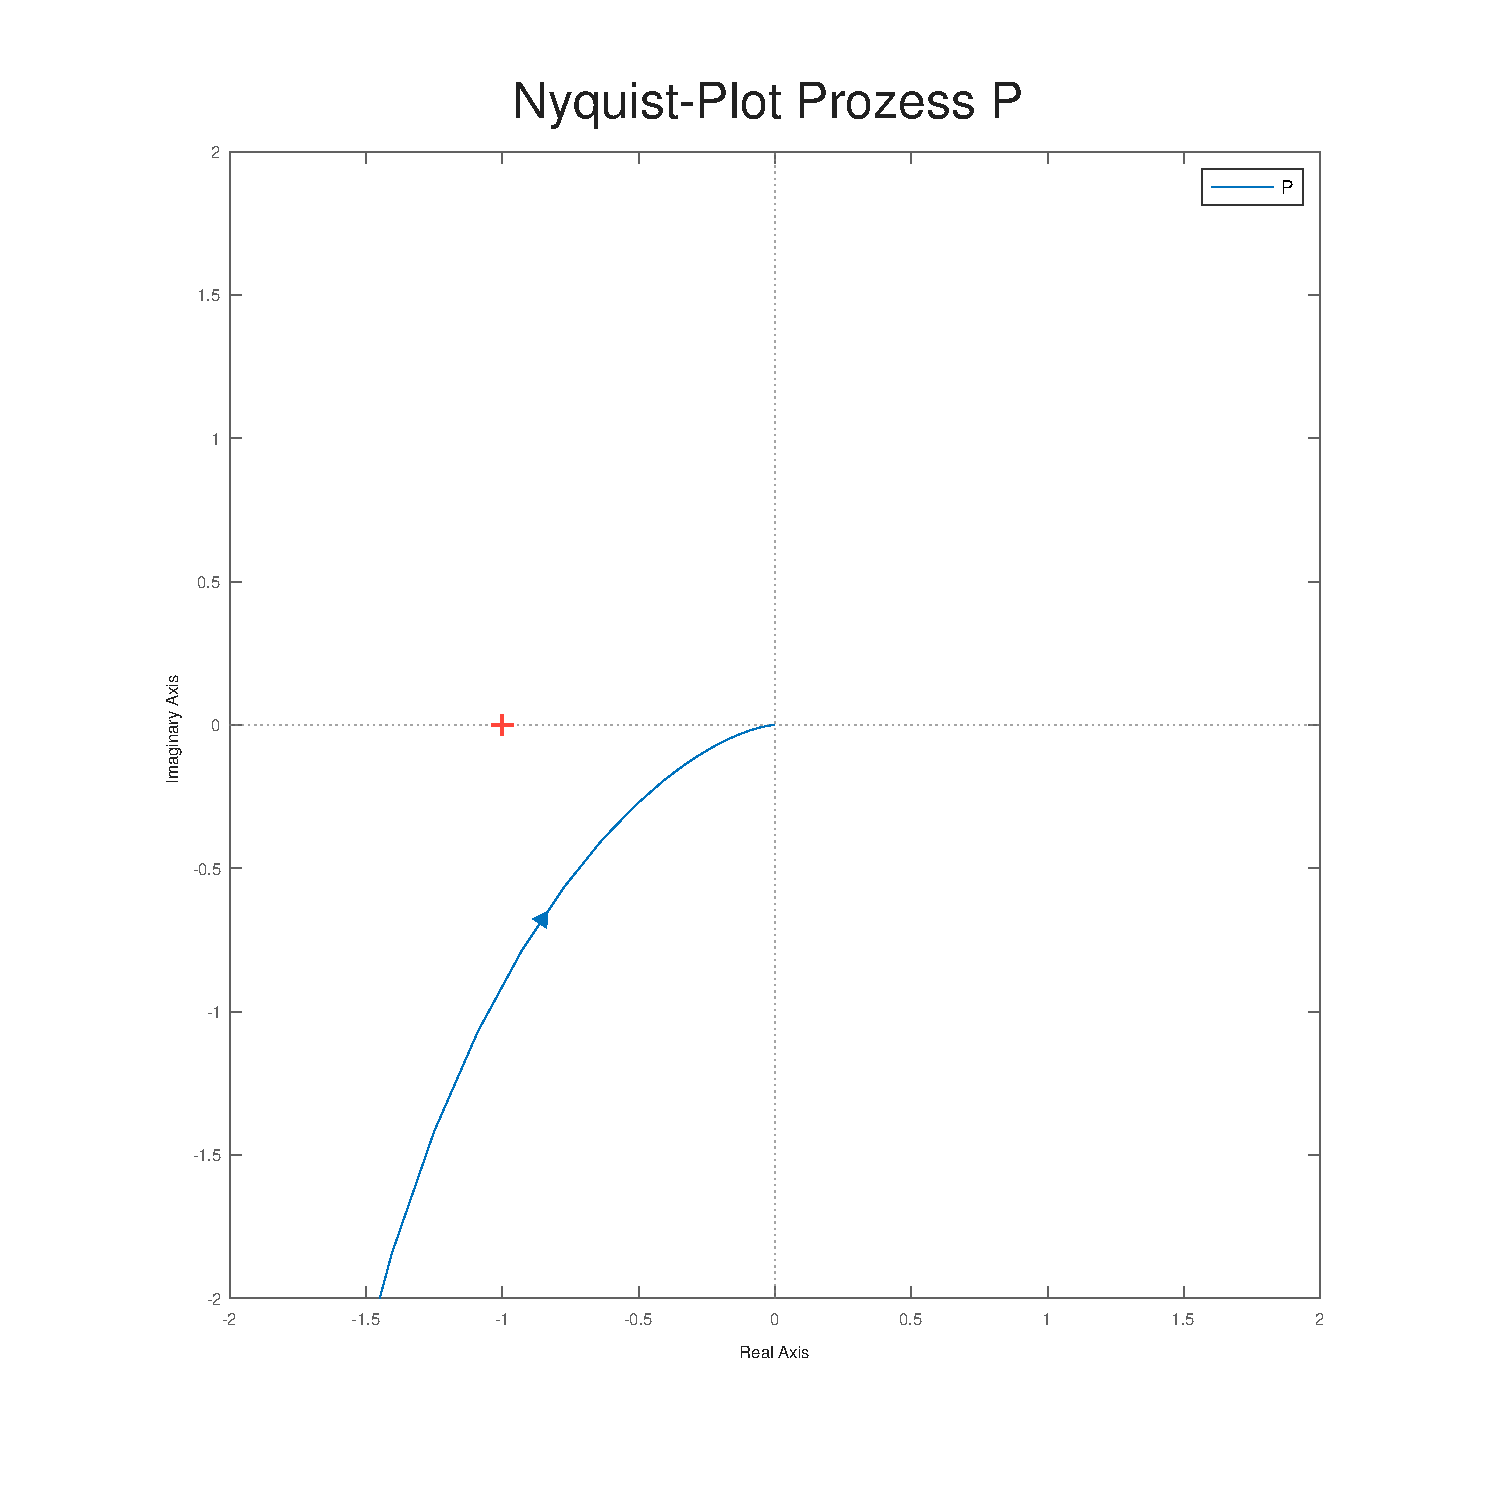
\includegraphics[width=0.75\linewidth]{fig_Parametrierung_Linienfolgeregler/NyquistPlot_System.pdf}
    \caption{Nyquistdiagramm des Prozesses $P(s)$}~\label{fig:Nyquist_raw}
\end{figure}

Abbildung~\ref{fig:MarginPlot_raw} zeigt den Bodeplot des Prozesses $P(s)$ mit
eingezeichneter Phasenreserve, während Abbildung~\ref{fig:Nyquist_raw} den
Nyquistplot des Systems zeigt.

\paragraph{Anforderungen an den Regler:} Das Einschwingverhalten des Prozesses sollte deutlich geglättet sein. Ein
einmaliges Überschwingen wird kaum vollständig zu vermeiden sein, jedoch sollte
der Regler innerhalb von $\approx 500 ms$ mindestens 90\% des Sprunges erreicht
haben. Damit ist der Regler in der Lage, das Fahrzeug innerhalb einer
\textit{minimalen Hindernisdistanz}, die in der FAQ mit 300mm angegeben ist,
mittig auf der Linie zu positionieren. Ein zwischenzeitliches Überschwingen von
20\% wird toleriert, da auf der Wettkampfstrecke in der Regel nicht mit
Sprüngen zu rechnen ist. Ein solcher Regler sollte daher völlig ausreichen, um
einer Linie geradeaus zu folgen.

\subsubsection*{Festlegung des Reglertyps und Parametrierung}

Die Abbildungen~\ref{fig:Nyquist_raw} und ~\ref{fig:MarginPlot_raw} zeigen,
dass der Prozess prinzipiell durch einen P-Regler mit der
Verstärkungskonstanten $k_p$ beschleunigt und stabil geregelt werden kann.
Durch die zentrische Streckung der Nyquist-Kurve nähert sich diese jedoch sehr
schnell dem rot markierten Punkt $-1$. Bei höheren Verstärkungen ist daher eine
Phasenanhebung erforderlich. Aus diesem Grund wurde ein PD-Regler gewählt. Am
Nyquistplot ist ersichtlich, dass ein allfälliger Integralanteil die Ortskurve
in Richtung $-1$ Punkt schieben würde, was die Stabilität des Systems
nachteiligt beeinflussen würde. Der Prozess an sich ist bereits integrierend,
was man an der Übertragungsfunktion sieht.

Der PD-Regler hat die Zeitkontinuierliche Form:
\[
    C(s) = k_p \cdot (1 + \frac{T_d \cdot s}{1 + \frac{T_d}{\alpha} \cdot s})
\]

Der Parameter $kp = 8$ wurde so gewählt, dass sich eine Phasenreserve von
$\approx 13^\circ$ ergibt. Um der sich daraus ergebenden Schwingung
entgegenzuwirken, ist der D-Anteil mit seiner Zeitkonstante $Td = 0.5s$ so
eingestellt, dass er genau im Bereich des $0 dB$ Durchtritts bereits eine
starke Phasenanhebung bewirkt.

Der D-Anteil des Reglers muss jedoch begrenzt bleiben, da die Systemantwort des
Reglers sonst in einem Dirac-Stoss enden würde. Der Parameter $\alpha = 8$ ist
so gewählt, dass der D-Anteil örtlich eher begrenzt bleibt. Der Sensor hat ein
starkes Rauschen. Wirkt der Regler zu stark differenzierend, wird sich das
Sensorrauschen stark im Systemverhalten des Roboters später widergeben. Der
Parameter $\alpha$ ist erst angenommen und später in Versuchen empirisch
optimiert.

Mit den Parametern $kp = 8$, $Td = 0.5$ \& $\alpha = 8$ kann also ein stabiles
System mit zügiger Sprungantwort erreicht werden. Der Phasen- und
Amplitudenverlauf sowie das aktualisierte Nyquist-Diagramm des geregelten
Prozesses sind in Abbildung~\ref{fig:MarginPlot_geregelt} und
Abbildung~\ref{fig:Nyquist_geregelt} dargestellt. Daraus ist auch jeweils das
Loop-Shaping im Vergleich zum Prozess ersichtlich.

\begin{figure}[H]
    \centering
    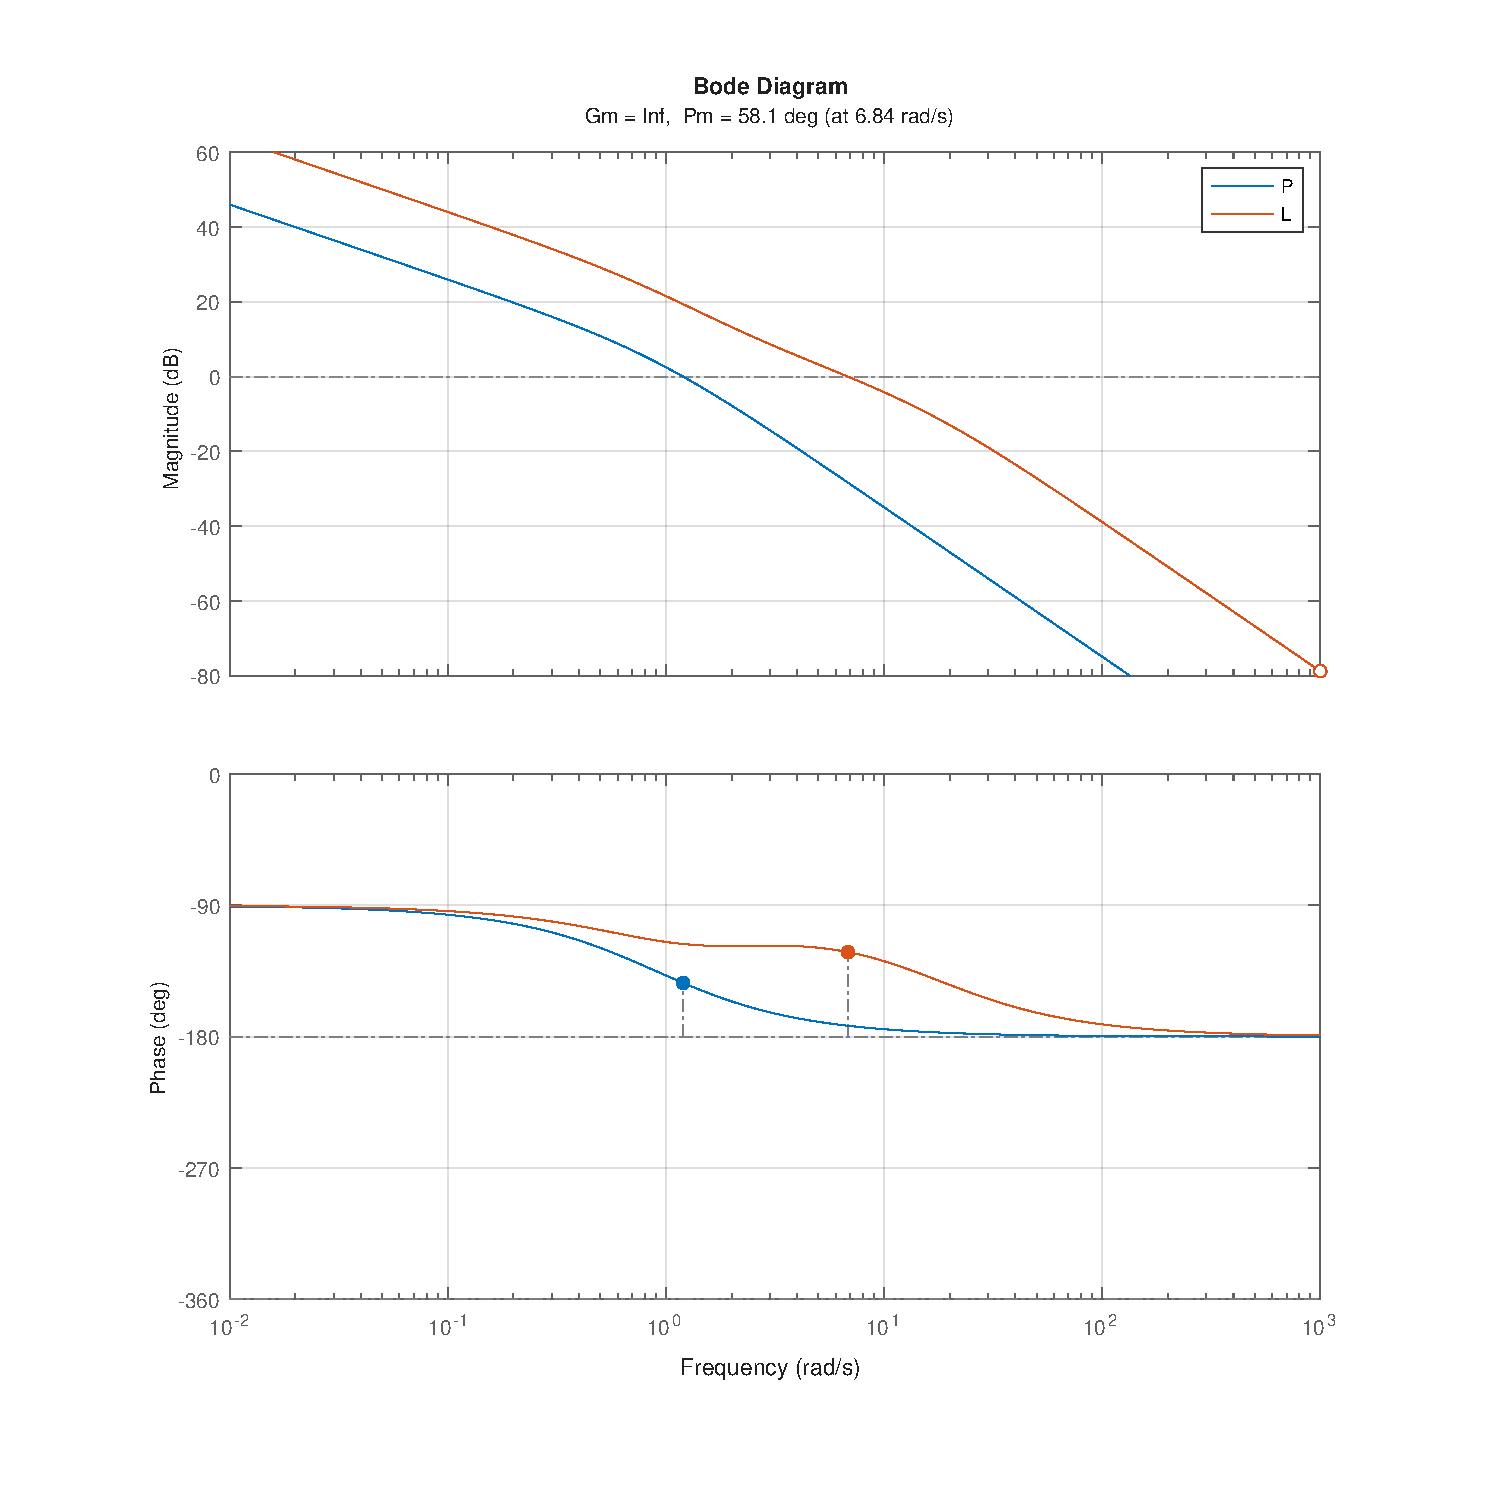
\includegraphics[width=1\linewidth]{fig_Parametrierung_Linienfolgeregler/Bode_Plot_Prozess_geregelt.pdf}
    \caption{Bodeplot mit eingezeichnter Phasen- und Amplitudenreserve des geregelten Prozesses}~\label{fig:MarginPlot_geregelt}
\end{figure}

\begin{figure}[H]
    \centering
    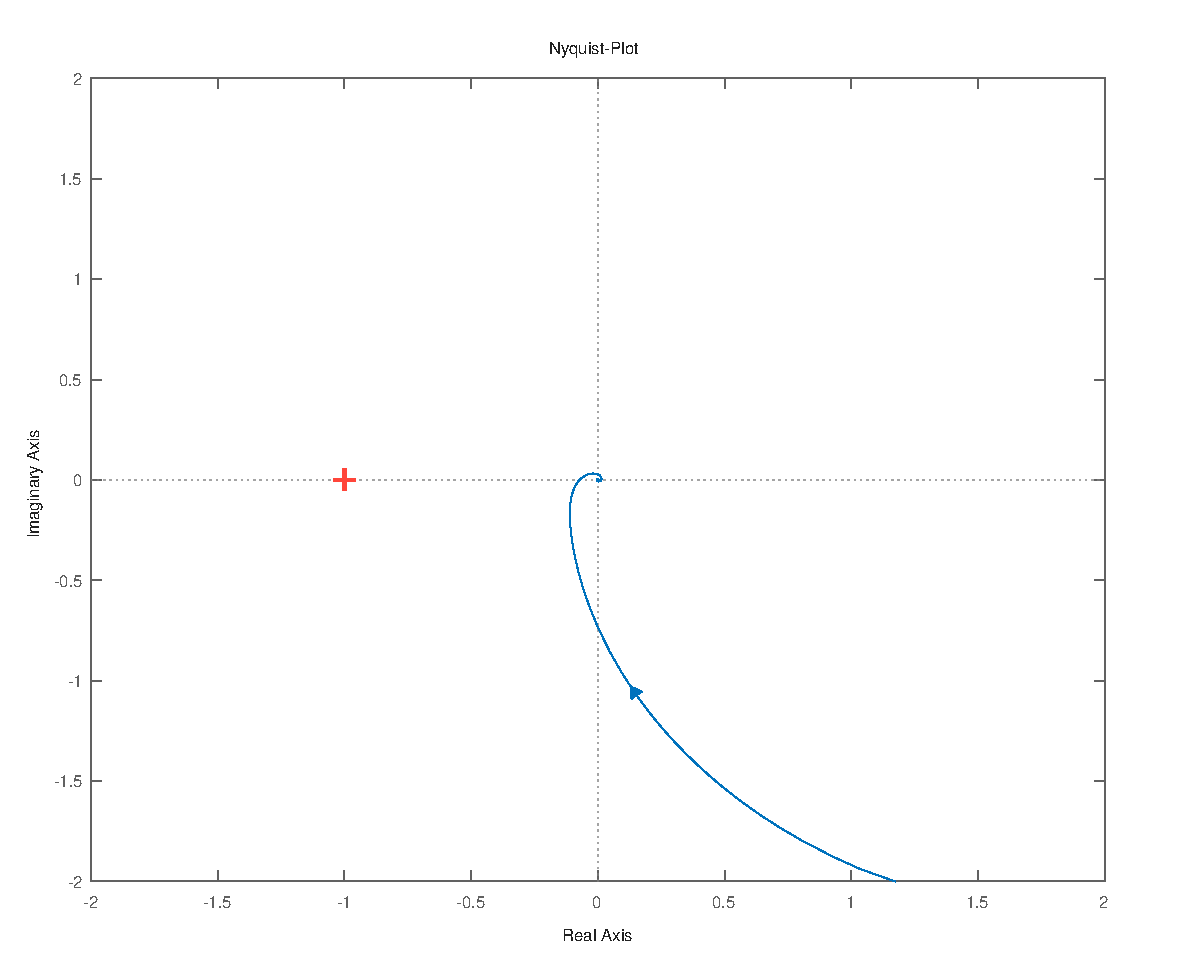
\includegraphics[width=0.75\linewidth]{fig_Parametrierung_Linienfolgeregler/NyquistPlot_System_geregelt.pdf}
    \caption{Nyquistdiagramm des geregelten Prozesses $P(s)$}~\label{fig:Nyquist_geregelt}
\end{figure}

\subsubsection*{Implementierung des Reglers in MotionController Firmware}

Mit Hilfe der \textit{Tustin-Approximation} kann der gefundene Regler
zeitdiskret approximiert werden. Es ergibt sich folgende Differenzengleichung
für den Regler $C(z)$.

\[
    u[k] = \alpha \cdot e[k] - \beta \cdot e[k - 1] + \gamma \cdot u[k - 1]
\]

Der Regler verwendet die Parameter $\alpha = 95.85$, $\beta = 58.67$ und
$\gamma = 0.0.8519$ und ist in der MotionController Firmware umgesetzt.

Ein erneuter Abgleich der Sprungantwort mit der Simulation in
Abbildung~\ref{fig:Sprung_geregelt} zeigt eine gute Annäherung, wobei die
Sprungantwort des Modells nicht ideal mit der Sprungantwort des realen Systems
zusammentrifft.

Die Abweichung lässt sich wahrscheinlich mit dem Rauschen des Liniensensor
erklären, wodurch der D-Anteil teils stark reagiert. Nichtsdestotrotz ist eine
sehr gute Reaktion auf den Sprung erreicht, welcher die gestellten
Anforderungen an den Regler erfüllt und sogar übertrifft.

\begin{figure}[H]
    \centering
    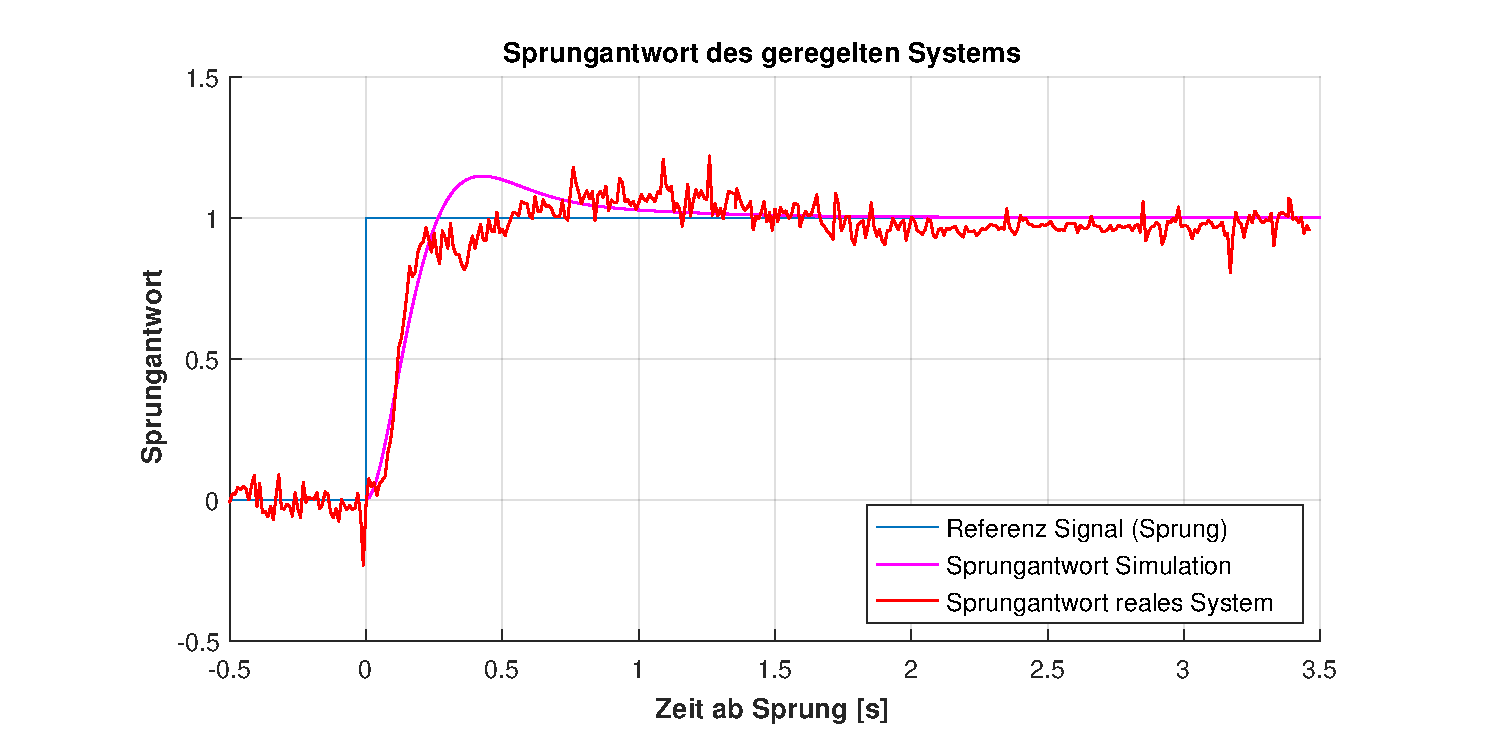
\includegraphics[width=1\linewidth]{fig_Parametrierung_Linienfolgeregler/Sprungantwort_System_kontrolle.pdf}
    \caption{Sprungantwort des geregelten Systems}~\label{fig:Sprung_geregelt}
\end{figure}

\end{document}